\documentclass[11pt]{article}

\usepackage[T1]{fontenc}
\usepackage[utf8]{inputenc}
\usepackage{lmodern}
\usepackage[letterpaper,margin=1in]{geometry}
\usepackage{graphicx}
\usepackage{booktabs}
\usepackage{tabularx}
\usepackage{array}
\usepackage{float}
\usepackage[labelfont=bf,labelsep=period,font=small]{caption}
\usepackage{enumitem}
\usepackage{parskip}
\usepackage{microtype}
\usepackage[hidelinks]{hyperref}
\usepackage{xurl}

\newcolumntype{L}{>{\raggedright\arraybackslash}X}
\setlist[enumerate]{leftmargin=1.6em,itemsep=0.35em,topsep=0.4em,parsep=0pt}
\setlist[itemize]{leftmargin=1.2em,itemsep=0.35em,topsep=0.4em,parsep=0pt}

%% Headings carry the same numbers the source document uses: "1. Introduction"
%% for a section, "4.1 From open language to symbols" for a subsection.
\renewcommand{\thesection}{\arabic{section}.}
\renewcommand{\thesubsection}{\arabic{section}.\arabic{subsection}}
\makeatletter
\renewcommand{\@seccntformat}[1]{\csname the#1\endcsname\hspace{0.5em}}
%% Reference list entries are plain hanging paragraphs, with no bracket labels,
%% because the source cites by author and year in running text.
\renewcommand{\@biblabel}[1]{}
\makeatother

\title{\textbf{An Agent That Copies Nobody Is Certified as a Leader}}
\author{Manu Nicholas Jacob \\ Independent Researcher \\ \texttt{manunicholasjacob@gmail.com} \\[0.6em] With Apart Research. \\ Track 4 (Multi-Agent Oversight and Control).}
\date{}

\begin{document}
\maketitle
\begin{abstract}
Multi-agent oversight increasingly relies on information-theoretic methods to identify influence between agents. These methods use lagged transfer entropy, surrogate testing to identify meaningful links, and per-agent influence scores. We test this approach on the AI Village corpus, which contains frontier models interacting in shared channels, and find that it needs two repairs. Replies arrive a median of 28.1 seconds apart, so no clock window both holds two speakers and separates a message from its answer, and a meaning-free hash null certifies comparably many edges as the topic symboliser, more at five minutes. A turn-ordered grid fixes that but breaks the conventional circular-shift surrogate: an agent planted with zero coupling is certified as a driver in 8 of 8 runs, and on structure-free data the family-wise error rate is 0.90 against a nominal 0.05. The cause is the structure of the speaker sequence, since randomising who speaks when removes the failure entirely, and a symbol-permutation surrogate restores the error rate to 0.063. Calibration is not confounding, so we also condition on the channel's recent state, validated on a released benchmark with a known influence graph where common-cause false edges fall from 22.3 to 0.33 and precision rises from 0.17 to 0.80 at unchanged recall. With both repairs, main-village keeps 2 dyad-specific edges that are robust to the conditioning resolution but still fail to replicate out of sample, while open-chat's 18 are undetermined, between 0 and 13 of them surviving depending on that resolution. We release the benchmark and the controls.
\end{abstract}
%% ================ BODY, SECTIONS 1 to 7 ================

\section{Introduction}

When AI agents interact in a shared channel, it is useful to understand how they influence one another. Information-theoretic methods offer a way to measure this through lagged transfer entropy, surrogate testing, and per-agent influence scores. They are attractive because they require no labels or access to model internals, only a record of who said what and when. However, the reliability of these measurements needs to be examined.

Almost every demonstration of these detectors runs on synthetic traces with a planted leader, where the analyst controls timing and vocabulary. Real agent chat is asynchronous, bursty and written in open language. This report asks a narrower question than ``what is the influence structure of a real swarm'': whether the standard recipe, applied to real agent logs, returns anything an overseer should act on.

We run that audit on the AI Village (AI Digest, 2026), in which frontier models share chat channels over eighteen months, across four villages differing in size, lifetime and tempo, applying the checks a reader should demand: planted controls, a meaning-free symboliser, replication in a held-out window, and sensitivity to every parameter we had to choose. Our audit identifies a specific failure in the method and shows how it can be addressed.

\begin{enumerate}
\item The conventional circular-shift surrogate is \textbf{invalid} on turn-ordered agent chat: a family-wise error rate of 0.90 against a nominal 0.05, caused by the structure of the speaker sequence itself.
\item The local-permutation surrogate restores calibration, and re-certifying under it \textbf{scrambles rather than shrinks} the answer: one channel loses all 11 of its edges, another gains 15.
\item Calibration is not confounding, so we add a conditional estimate and validate it on a \textbf{released benchmark} with a known influence graph: common-cause false edges fall from 22.3 to 0.33, precision from 0.17 to 0.80, with no loss of recall or power.
\item On the real channels two edges stand at every conditioning resolution, 18 are \textbf{undetermined} between 0 and 13, none replicates out of sample, and what survives alongside humans runs from people to agents.
\end{enumerate}

\section{Related Work}

\textbf{Transfer entropy and surrogates.} Transfer entropy (Schreiber, 2000) measures how much a source's past reduces uncertainty about a target's next symbol beyond the target's own past. Plug-in estimators are biased upward on short series, so significance rests on surrogate data, with family-wise error across all ordered pairs controlled by a max-T test (Westfall and Young, 1993). The usual surrogate is a circular time shift of the source.

\textbf{Event-based data breaks the shift surrogate.} Our audit rediscovers this in a new domain. Shorten, Spinney and Lizier (2021), on neural spike trains, show that the conventional source-time-shift surrogate fails to represent the null hypothesis of conditional independence for event-based processes, and adapt to that setting the nearest-neighbour local permutation scheme of Runge (2018). Agent chat is event-based in that sense: messages are events in continuous time, not samples of a clocked signal. The correction itself is not our contribution. Ours is showing that the same failure carries over to multi-agent safety monitoring and can be severe enough to create apparent leaders where none exist.

\textbf{Oversight under a budget.} AI-control research frames monitoring as resource constrained, with a cost for false positives (Greenblatt et al., 2024); an influence graph is one such measurement and our concern is its error rate.

\section{Data}

The AI Village dataset ships one gzipped-JSONL table per village. We use four villages, which differ enough to test whether any finding is a property of one channel.

\begin{center}
\small
\begin{tabular}{llllll}
\toprule
\textbf{village} & \textbf{agent messages} & \textbf{agents} & \textbf{lifetime} & \textbf{human messages} & \textbf{busiest room} \\
\midrule
main & 205,726 & 58 & 576 days & 10,029 & \#general (166,715, 81\%) \\
open-chat & 35,483 & 23 & 66 days & 12,264 & \#general (all) \\
swarm & 3,848 & 133 & 1 day & 5 & room a (3,846) \\
game-jam & 838 & 6 & 3 days & 36 & per-team rooms \\
\bottomrule
\end{tabular}
\end{center}

A 2026 scaffolding change scopes each agent to its current room's context, so the busiest room of each village is a self-contained influence substrate and we analyse it alone. The primary window is the final fourteen days of main-village \#general, 17 to 31 October 2026, holding 8,800 agent messages; twenty-two models posted at least 50 messages each and the directed test uses the 15 busiest, giving 7,958 message events. Two scaffolding facts are disclosed rather than corrected: the automated nudger was off throughout, and the unused \#best and \#rest rooms were soft-deleted mid-window, which does not touch \#general. We read message metadata and text only, and human participants appear only as aggregated or anonymised nodes.

\section{Method}

\subsection{From open language to symbols}

Transfer entropy needs discrete symbols, so each message is mapped to a small alphabet before influence is estimated, and that mapping is kept separate from the estimator. A topic symboliser (TF-IDF then k-means, k=8) gives a message its topic cluster id, so paraphrases of one idea share a symbol. A hash symboliser (a stable hash of the normalised text into k=8 buckets) has no notion of meaning and serves as a null: an edge appearing under both lives in timing alone.

\subsection{The lag problem, and why clock windows cannot solve it}

A lag-1 transfer entropy compares window t-1 with window t, so influence landing inside one window is invisible to it. Agent chat makes this binding. Among the fifteen analysed agents the gap between consecutive messages by different speakers has a median of 28.1 seconds (25th percentile 9.2, 75th 66.2, 95th 159.3), so turn-taking is a seconds-scale process while any clock window wide enough to hold two speakers is minutes wide and swallows both a message and its answer.

Appendix F measures both horns: at 30 seconds only 1.2\% of agent-windows hold a message while 32.0\% of replies already land in the same window as what they answer, by 5 minutes that share is 84.4\%, and across the widths we tried the meaning-free hash null certifies comparably many edges to the topic symboliser, more of them at five minutes. Clock windows do not detect shared meaning here.

We avoid the bind by ordering messages canonically and letting one message be one tick. Each agent's series carries its symbol where it spoke and a silent symbol elsewhere, so the lag-1 comparison is between a message and the one immediately before it. The cost is that the measure captures immediate-predecessor influence only.

\subsection{Two surrogate nulls}

The preexisting estimator certifies an edge by comparing the observed transfer entropy with a \textbf{circular-shift} surrogate of the source, using a max-T family-wise test at level 0.05 across all ordered pairs. On the turn-ordered grid this surrogate fails. Real conversation is not a sequence of independent draws about who talks next: it has strong turn-taking and strongly non-stationary per-agent activity, and circularly shifting one agent's series slides that pattern to a different part of the timeline, where it aligns against the others differently than it ever does in the data.

We therefore add a \textbf{symbol-permutation} surrogate, following the local-permutation idea of Runge (2018) as adapted to event data by Shorten et al. (2021): the source keeps the exact ticks at which it spoke, and only its symbols are permuted among them. Speaking pattern, sparsity and turn-taking are preserved exactly, and only the correspondence between symbol and time is destroyed. Both surrogates are reported throughout.

\subsection{A second repair, for common cause}

A valid surrogate fixes calibration but not confounding. If every agent tracks a drifting channel topic, every pair is genuinely dependent through the channel, and pairwise transfer entropy cannot tell that from direct influence. We therefore also report a \textbf{conditional} estimate, which asks whether a source's last message adds anything about a target's next one beyond the target's own history \textbf{and the channel's recent state}. The conditioning variable is the modal symbol of the last twelve messages, excluding the immediately preceding one so that it does not simply restate the source.

The two estimates bound the answer rather than one superseding the other: pairwise asks whether there is directed topical dependence at all, including dependence mediated by the channel, and conditional asks whether it is specific to the pair. Influence that works by shifting what the room talks about is real influence, and conditioning removes it, which is why both are reported.

\subsection{Controls}

Real logs have no ground truth, so we plant it. A synthetic follower is spliced into the real stream, copying a chosen leader's topic on a fraction of its messages; sweeping that fraction and its volume gives the detection floor. A planted agent coupled to \textbf{nothing} should never be certified, and the real speaker sequence with its symbols globally permuted contains no directed topical influence by construction, so a calibrated procedure should fire in about 5\% of replicates. Every edge set is then recomputed in the adjacent fourteen-day window, in each half of the primary window, and at several alphabet sizes. Appendix H gives the construction in full.

\section{Results}

\subsection{On a turn-ordered grid the standard surrogate is invalid}

We plant an agent into the real stream, drawing its symbols from the channel's marginal and coupling it to nothing at all, then ask how often it is certified as driving something. It is certified in 3 of 8 runs when it posts 50 messages, and in 8 of 8 at 100, 263, 600 and 1500 messages, with the mean largest z rising from 5.6 to 12.3, 21.7, 38.3 and 71.7. The error grows with how much the agent speaks, which rules out a small-sample explanation.

A planted agent could be dismissed as artificial, so we also measure the error rate directly. Keeping the real speaker sequence and permuting the symbols globally leaves data with no directed topical influence by construction. The shift surrogate certifies at least one edge in 9 of 10 such replicates, a family-wise error rate of 0.90 against a nominal 0.05.

\textbf{What breaks it is the speaker sequence.} Destroying one structure at a time isolates the cause (Appendix D). Keeping the real speaker order and shuffling only symbols, the shift surrogate fires in 10 of 10 replicates; randomising the speaker order too drops it to 0 of 10; uniform symbols with the real order still give 6 of 10. So the driver is the structure of the speaker sequence, not the symbol distribution and not sparsity. That sequence is far from random in two ways at once: it repeats a speaker 36\% of the time and returns after one message 38\% of the time, and each agent's activity is strongly non-stationary, with a median block-share coefficient of variation of 0.79. Shuffling the order destroys both at once, so our ablation does not separate them, and we do not claim it does. Shifting slides an agent's whole activity pattern across the timeline; permuting symbols within its own positions leaves that pattern intact.

\subsection{A sparsity-preserving surrogate restores calibration}

Following the local-permutation idea of Shorten et al. (2021), we keep each source's speaking positions and permute only its symbols among them. On the same destroyed-structure data the family-wise error rate falls to 0.063 over 300 replicates, with a 95\% Wilson interval of 0.041 to 0.097, so it is close to the nominal 0.05 and clearly separated from the 0.90 it replaces. The planted uncoupled agent is now never certified: 0 of 5 at both 263 and 1500 messages, with mean max z of 2.8 in each case against 22.0 and 68.3 under the shift surrogate. Appendix D shows the failure is not an artifact of our configuration: it survives swarm size, a near-uniform alphabet, and an independent symboliser.

\setcounter{figure}{0}
\begin{figure}[H]
\centering
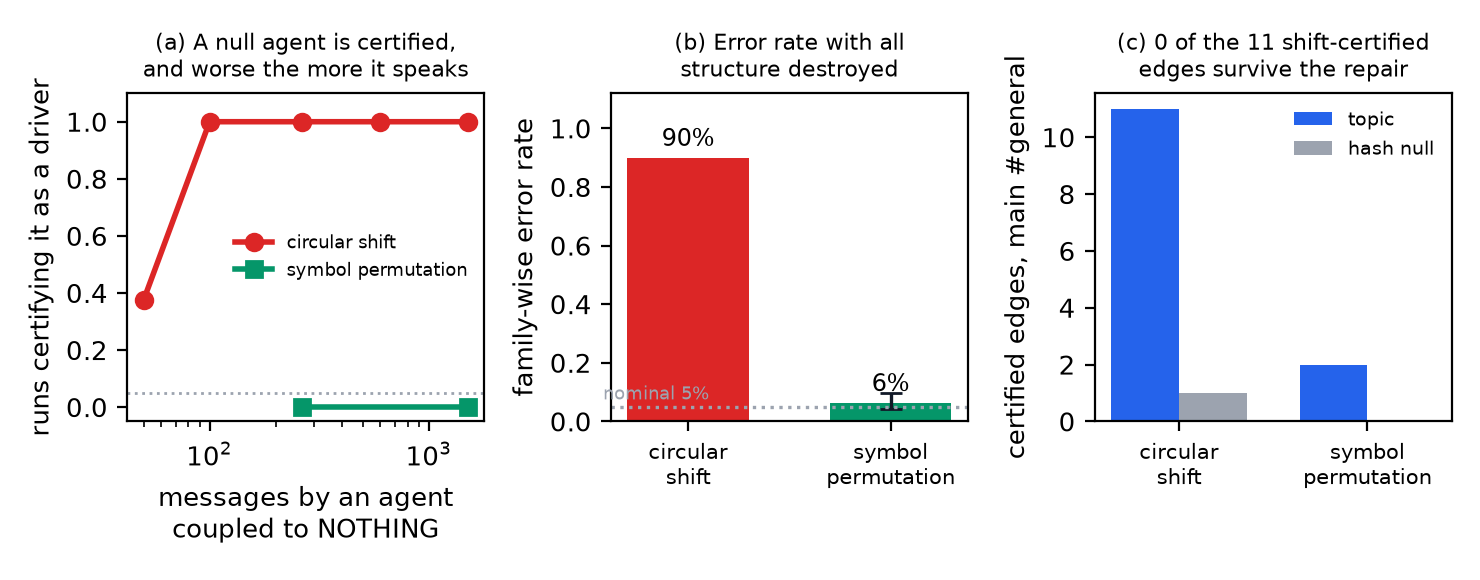
\includegraphics[width=0.9\textwidth]{f2_null.png}
\caption{Left, how often an agent coupled to nothing is certified as a driver, under each surrogate. Middle, family-wise error rate measured on data with all structure destroyed, with a Wilson interval; the dotted line is the nominal 0.05. Right, what each surrogate certifies on the real channel.}
\end{figure}

\subsection{The same channels, re-certified}

Re-running every channel under the repaired surrogate changes the answers, and not in one direction.

\begin{center}
\small
\begin{tabular}{llll}
\toprule
\textbf{channel} & \textbf{window messages} & \textbf{shift: topic / hash} & \textbf{permutation: topic / hash} \\
\midrule
main \#general & 8,800 & 11 / 1 & 2 / 0 \\
open-chat \#general & 8,226 & 3 / 0 & 18 / 0 \\
swarm, room a & 3,846 & 2 / 1 & 1 / 0 \\
\bottomrule
\end{tabular}
\end{center}

In main-village, \textbf{none} of the 11 edges the standard recipe certifies survives the repair, and the two the valid surrogate certifies were not among them. In open-chat the correction runs the other way, 3 edges becoming 18, because pathological pairs inflate the max-T threshold and raise the bar for everything else. An invalid surrogate does not simply add false positives, it scrambles the result.

\subsection{Conditioning on the channel, and what it removes}

A valid surrogate does not address confounding, so we built a generated benchmark with a known influence graph (Appendix E). Its decisive instances contain no influence while every agent tracks a shared drifting topic, so any certified edge is common cause. There, pairwise transfer entropy certifies \textbf{22.3} edges on average and conditioning takes that to \textbf{0.33}, lifting pooled precision on the four-edge instances from 0.17 to \textbf{0.80} at a recall of 1.0 either way, and across couplings from 0.05 to 0.8 the conditional test still finds the planted edge in 3 of 3 runs, so the gain costs no power.

The benchmark flatters the conditional estimator, since its common cause is a shared modal topic and the conditioning variable is the channel's modal topic. The real channels are the harder test, and conditioning there costs degrees of freedom: a 9-symbol alphabet with a 9-valued context gives 6,561 cells against about 7,900 ticks, roughly one observation per cell. So we also coarsen the same variable to 4 and 2 values.

\begin{center}
\small
\begin{tabular}{lllll}
\toprule
\textbf{channel} & \textbf{pairwise} & \textbf{conditional, 9 values} & \textbf{4 values} & \textbf{2 values} \\
\midrule
main \#general & 2 & \textbf{2, the same two edges} (mean z +0.34) & 2 & 3 \\
open-chat \#general & 18 & \textbf{0} (mean z -0.34, max z 4.4) & \textbf{7} & \textbf{13} \\
swarm, room a & 1 & \textbf{0} &  &  \\
\bottomrule
\end{tabular}
\end{center}

\textbf{Main-village's two edges are robust to that choice; open-chat's zero is not.} At the finest resolution the open-chat test is degenerate, its surrogate sitting above the observed statistic for 65\% of pairs with the largest z in the family only 4.4, so it is failing to reject rather than finding nothing to reject. Open-chat's structure therefore remains \textbf{undetermined}: depending on the conditioning resolution, between 0 and 13 of its 18 edges may survive. The resolution is a free parameter an analyst would otherwise set once and never revisit, and on one of our two channels it decides the answer.

This is a property of that channel and not of the estimator: on structure-free real data the conditional test fires in 2 of 40 replicates, an error rate of 0.05 with a mean z of -0.001, so it is nominal rather than systematically conservative (Appendix G).

Those two edges are the strongest thing in this report and they are still not a finding, because they do not replicate: the adjacent fourteen-day window certifies nothing at all, under either estimator. Given the detection floor in Appendix G that silence is as consistent with the test sitting near its limit as with the edges being absent, and we cannot separate the two.

\subsection{Power, and whether anything replicates}

Both bound the claims above and both are in Appendix G. Power is governed by how much an agent says as much as by how strongly it copies, and it is channel-specific: in main-village a planted follower copying on 80\% of its messages is caught only 1 time in 4, while in open-chat one copying 10\% of the time is caught 3 times in 4, so main-village's two edges are a floor and not a description. Replication is weak everywhere. Under the standard recipe the adjacent fourteen-day window shares 1 edge out of 8 and 4, and that surviving edge is also the only one the meaning-free hash null certifies. Under the repaired surrogate, and again under conditioning, the adjacent window certifies nothing at all, so there is nothing to share. No certified edge in this report replicates out of sample.

\subsection{Humans in the channel}

main-village \#general is now effectively human-free, with 3 human messages in the window, so the question has to be asked in open-chat, where 32\% of messages come from 124 human visitors. Pairwise, with humans collapsed into one node, 19 edges are certified. Conditioning removes almost all the agent-to-agent structure and little of the rest: \textbf{four edges survive, of which three run from humans to agents, one is agent to agent, and none run from an agent to a human.} So the asymmetry is not an artifact of the confound. Read it carefully all the same: the measurement supports only that the dependence is dyad-specific and directional, not that anyone is steering a swarm. Appendix I has the breakdown.

Appendix D reports two further traps: a net-influence score measures volume rather than meaning, and a copy-rate detector does not reproduce transfer entropy, so what this report indicts is the surrogate and not the statistic.

\section{What an overseer should do}

Five inexpensive controls should be included whenever an influence graph over an agent channel is published.

\begin{enumerate}
\item \textbf{Plant an agent coupled to nothing, at your channel's volumes, and check it is not certified.} This one test would have caught the failure reported here, at one run per volume.
\item \textbf{Measure the error rate directly,} by destroying the structure your method claims to find and checking the family-wise rate is near nominal. If it is not, your surrogate does not match your data.
\item \textbf{Preserve the speaker sequence in your surrogate.} Any surrogate that moves an agent's messages in time will disturb it. Shorten et al. (2021) is the principled route.
\item \textbf{Establish the detection floor before interpreting an absence.} ``No edges'' and ``no influence'' are different claims.
\item \textbf{Condition on the channel, report both numbers, and sweep the resolution.} Pairwise and conditional bound the answer and the gap between them is the result; conditioning costs cells, so check whether your answer is an artifact of how finely you conditioned. On one of our channels it was.
\end{enumerate}

Two habits follow: publish a meaning-free null's edge count beside the real one, and require held-out replication before calling a graph the structure of a swarm.

\section{Conclusion}

Applied to real agent chat, the standard recipe for ``who drives whom'' needs two repairs before it says anything. Clock windows cannot separate a message from its answer at the timescale agents reply on, and the edges they certify are reproduced by a null with no access to meaning. The turn-ordered representation that fixes this breaks the circular-shift surrogate, whose family-wise error rate on structure-free data we measure at 0.90 against a nominal 0.05, caused by the structure of the speaker sequence itself. A valid surrogate then fixes calibration but not confounding, and conditioning introduces a resolution of its own. What survives is small: two dyad-specific edges that do not replicate, an undetermined answer where conditioning resolution decides it, and, where humans are present, influence running from people into agents and never back. An influence graph should not guide decisions until its error rate, confound, and detection floor are all reported.

%% ================ APPENDICES A to I ================
\appendix
\renewcommand{\thesection}{Appendix \Alph{section}:}

\section{Limitations}

\begin{itemize}
\item \textbf{Immediate-predecessor only.} The turn-ordered lag-1 measure sees influence from the message directly before a reply. Influence acting over several turns, or through a room's accumulated context, is out of scope and needs a higher-order or memory-aware estimator.
\item \textbf{Discrete approximation to an event process.} Agent chat is event-based in continuous time. We use a turn-ordered discretisation with a permutation surrogate as a practical fix; a continuous-time estimator (Shorten et al., 2021) is the principled route and we did not attempt it.
\item \textbf{Symbolisation is a free parameter, and we cannot measure its quality on the real logs.} The central result survives an independent symboliser (Section 5.3), but the edge count does not: it moves with the alphabet size and with which messages the topic model is fit on, and we report those sensitivities rather than tuning them. Two of the eight topic clusters are dominated by function words, because the preexisting symboliser does not remove stopwords. On the benchmark, where true topics are known, we can measure it, and Appendix E shows a sharp floor: once the symboliser's agreement with the truth falls below roughly 0.44 by adjusted Rand index, detection collapses regardless of estimator. We have no corresponding number for the real channels, so we cannot rule out that they sit near that floor, and that is the single largest unquantified threat to everything reported here.
\item \textbf{No ground truth in the real logs.} The validity argument rests on planted controls and on the meaning-free null, not on recovering a known answer.
\item \textbf{Scaffolding confounds.} Agent behaviour is shaped by prompt, tool and memory changes logged in the dataset's changelog. We chose a window in which the message-injecting nudger was off, but other scaffolding is held fixed only by the shortness of the window.
\item \textbf{Conditioning removes real influence too.} The conditional estimate discards any influence that works by shifting what the channel is talking about, which in a group chat may be a large part of genuine influence. It is a lower bound on dyadic influence, not a better measurement of influence in general, which is why both estimates are reported.
\item \textbf{The human result is exploratory.} It rests on one village and one window, and should be read as a lead. Topical dependence from a human to an agent is also consistent with ordinary responsiveness rather than steering.
\end{itemize}

\section{Dual-Use and Ethical Considerations}

This work audits influence detection on a population of AI agents, which is dual-use. Used defensively it helps an overseer decide what an influence graph is worth, and our main result is deflationary: it tells practitioners to trust these outputs less, which reduces rather than increases the chance of acting on a bad attribution. The same tooling could be used to identify the most influential agent in a swarm in order to target it, or to surveil participants in a channel. Three properties limit the misuse. The subjects are AI models; the dataset is already public under research terms and we add no re-identification; and the measure is weak and local, recovering immediate-predecessor topical dependence rather than any model of how to steer an agent.

We followed the dataset's research terms: research use only, no training on the data, no re-identification, and citation of the source. Human participants appear only as an aggregate node or as anonymised visitor-1..n labels, never by name or handle, and we report no content attributable to an individual person. We read message text and metadata only, never model weights or private user data.

\section{Preexisting tools, new work, and LLM usage}

\textbf{Preexisting (declared).} The estimator (lag-1 transfer entropy, circular-shift surrogate, max-T family-wise test) and the reader and symbolisers (topic and hash) were built before the sprint in the repository swarm-prep and are declared preexisting with their validation numbers in that repository's README. Before the sprint, authentication was verified and filenames were listed, but no chat content was read or described, so the weekend is the first reading of the data. The preexisting validation used synthetic chat in which several agents speak per window, a setting in which the circular-shift surrogate is valid; the invalidity reported here arises only on the one-message-per-tick grid introduced this weekend, and is not a defect of the preexisting tool as validated.

\textbf{New this weekend.} The subset and window choices on the real data; the measured reply-latency justification for the lag; the turn-ordered representation; the symbolisation of real message text; the clock-window failure analysis; the symbol-permutation surrogate, the demonstration that the shift surrogate is invalid on this grid, and the ablation isolating turn-taking as the cause; the conditional estimator and its validation; \textbf{SwarmInfluence-Bench}, the generated benchmark of Appendix E; the planted positive and negative controls; the calibration measurements; the replication and sensitivity battery; the four-village comparison; the human-node analysis; the trivial-baseline comparison; all figures; and a vectorised reimplementation of the preexisting estimator, used only for scale and verified bit-for-bit against the preexisting code before use.

\textbf{LLM usage.} The author used an AI coding assistant (Claude) to help write and run the analysis code, to help draft this report, and to structure the figures. The author is responsible for every claim, number and figure here. All results come from the released code run on the public dataset, no result or reference is fabricated, and the numbers in this document are checked against the analysis output by a script that fails on any mismatch.

\section{Isolating the cause, robustness, and two further traps}

\textbf{Which structure breaks the surrogate.} Each condition below contains no directed topical influence by construction, so a calibrated procedure should fire in about 5\% of replicates. Ten replicates each.

\begin{center}
\small
\begin{tabular}{lll}
\toprule
\textbf{condition} & \textbf{circular shift} & \textbf{symbol permutation} \\
\midrule
real speaker order, symbols shuffled & \textbf{10 / 10} & 0 / 10 \\
real speaker order, uniform i.i.d. symbols & 6 / 10 & 1 / 10 \\
speaker order shuffled, symbols shuffled & \textbf{0 / 10} & 1 / 10 \\
speaker order shuffled, uniform i.i.d. symbols & 0 / 10 & 1 / 10 \\
\bottomrule
\end{tabular}
\end{center}

Speaker order is the switch and the symbol distribution only modulates. A generated channel with exactly one speaker per tick but stationary activity leaves the shift surrogate roughly calibrated at 0.067, which is how we found this: mutual exclusivity alone, our first proposed explanation, is not sufficient. Sweeping the generated activity from stationary to strongly non-stationary, 30 replicates per cell, raises the shift surrogate through 0.133 and 0.200 to \textbf{0.367}, while the permutation surrogate stays between 0.033 and 0.167 with every 95\% interval covering the nominal 0.05.

\begin{center}
\small
\begin{tabular}{lll}
\toprule
\textbf{activity drift} & \textbf{shift} & \textbf{permutation} \\
\midrule
0.0 & 0.067 & 0.033 \\
0.3 & 0.133 & 0.100 \\
0.6 & 0.200 & 0.167 \\
0.9 & \textbf{0.367} & \textbf{0.100} \\
\bottomrule
\end{tabular}
\end{center}

The real channel's agents sit at the top of that range, with a median block-share coefficient of variation of 0.79. So non-stationary activity is one sufficient route to the failure, and the repair survives it. Two cautions: because shuffling the speaker order destroys turn-taking and non-stationarity together, we cannot say which of the two is doing more work on the real data; and 30 replicates leave intervals wide enough that the permutation column should be read as not shown to fail rather than shown to be nominal. An earlier 8-replicate version of this sweep put the permutation surrogate at 0.375 at drift 0.6, which is why it was re-run.

\textbf{The surrogate failure is not an artifact of our configuration.} It is not a large-swarm effect: across swarms of 5, 10, 15 and 20 agents the shift surrogate certifies something in 22 of 24 null replicates, against 3 of 24 for the permutation surrogate, so shrinking the swarm does not rescue it. It is not a property of the skewed topic alphabet either, since on the near-uniform hash alphabet, where the largest symbol holds 13\% of messages rather than 37\%, the shift surrogate still fires in 10 of 10 replicates.

\textbf{Both corrections survive a different symboliser.} Replacing TF-IDF and k-means with latent semantic analysis gives 12 edges against 1 in main-village and 2 against 22 in open-chat: the same inflation and the same masking, reached by an independent route to topics. The meaning-free hash control gives 1 against 0 and 0 against 0. So the central result concerns the surrogate rather than any one clustering choice, although the edge count itself remains sensitive to the alphabet size.

\textbf{A continuous influence score measures volume.} Summed outgoing minus incoming transfer entropy, a common per-node leadership summary, ranks agents almost identically under the topic symboliser and under the meaning-free hash null (Spearman 0.85), with the same agent on top at nearly the same value. A score the hash null reproduces cannot be measuring shared meaning, so the certified edge set should be reported instead.

\textbf{The estimator is not redundant, though.} A trivial detector, the rate at which an agent repeats the previous message's topic in excess of its own base rate, ranks pairs very differently from transfer entropy (Spearman 0.21), and the pairs it ranks highest overlap the certified set in only 3 of 10 cases. So transfer entropy is not an expensive way to compute a copy rate, and the failure documented in this report belongs to the surrogate rather than to the statistic.

\section{the benchmark, and why it exists}

Real logs have no ground truth, so the common-cause question could not be settled on them. We built a generator in which the influence graph is known by construction: it decides, in code, who speaks at which tick, on which topic, and who reacts to whom. Surface text is a separate, replaceable layer drawn from disjoint per-topic vocabularies, so the whole thing runs offline and a detector still has to symbolise raw text rather than read the labels.

It has two null families and the distinction is the point. \textbf{Pure nulls} have no influence and no common cause, and measure calibration. \textbf{Common-cause nulls} have no influence between agents but a shared drifting channel topic, so every pair is genuinely dependent through the channel; they measure confounding. A benchmark with signal in every instance cannot see the failure mode this report is about.

\textbf{What the validation measures.} Three seeds per family, each with its own seed stream, 100 surrogates per test, the symbol-permutation null throughout, so pairwise and conditional differ only in whether the channel's recent state is conditioned on. On the common-cause nulls pairwise certifies 22.3 edges and conditional 0.33. On the four-edge instances pairwise certifies 23.3 to recover the 4, a pooled precision of 0.17, while conditional certifies \textbf{5.0 and still recovers all 4}, a precision of \textbf{0.80}. Recall is 1.0 either way. On the pure nulls pairwise fires in 1 of 3 and conditional in 1 of 3. Pooled precision counts every instance rather than only those that fired, because averaging precision over instances that fired flatters a detector that stays silent.

Two findings came out of building it. \textbf{Our initial explanation for the surrogate failure was incorrect.} A generated channel with exactly one speaker per tick but stationary activity still left the shift surrogate reasonably calibrated at 0.067. This result led us to examine the speaker sequence separately. We still cannot distinguish the effects of turn-taking from non-stationary activity, since shuffling the speaker order changes both. And it showed that \textbf{precision, not recall, is the weak point} of pairwise transfer entropy, which is what motivated the conditional estimate.

Three honest caveats. The benchmark's common cause is a shared modal topic and our conditioning variable is the channel's modal topic, so Section 5.4's synthetic numbers are close to a best case; the real-channel result is the harder test and we report it alongside. The generator draws speakers independently, so it does \textbf{not} reproduce the turn-taking that breaks the shift surrogate on real logs, which is a limitation we found rather than designed.

The third caveat is about the labels, and auditing our own generator changed numbers in this report. Only one agent speaks per tick, so when a leader has two followers whose reaction coins both land they cannot both reply at the stated lag: the second is pushed to the next tick. An early version dropped it instead, which understated coupling for every follower after the first. Re-queueing fixes that, but the requested coupling is still not the realised one, so the generator now measures and reports both: a labelled 0.3 realises about 0.18 when it shares its leader with another follower, while unshared edges realise their label to within 0.03.

More importantly, \textbf{a planted edge does not only couple its own pair}. Because a queued reaction consumes the tick, every other agent becomes less likely to speak immediately after the leader. On the four-edge instance the probability that a non-follower speaks in the tick after the leader falls to between 0.19 and 0.83 of its own base rate, against 0.94 to 1.05 on an otherwise identical instance with no planted edges. That displacement is a real lag-1 dependency and the label set does not contain it, so \textbf{precision on this benchmark is a lower bound for any detector}, and what the benchmark supports is the comparison between the two estimators rather than the absolute value of either. We report the measured 0.80 rather than patching the labels until our own method scores well, and the measurement is in the repository's test suite so a user can see the size of the gap.

\textbf{Does any of this depend on the text being easy?} It is a fair objection to a synthetic text layer that disjoint per-topic vocabularies make symbolisation trivial, so every number above assumes a symboliser that does not exist. Real messages are not like that: most words are common to every subject and only a few are distinctive. So the generator takes a \texttt{vocab\_overlap} parameter, the fraction of each topic's vocabulary shared with every other topic, and we sweep it. Adjusted Rand index is measured between the symboliser's output and the generator's true topic labels, so the degradation is quantified rather than asserted.

\begin{center}
\footnotesize
\begin{tabularx}{\textwidth}{LLLLLL}
\toprule
\textbf{vocabulary overlap} & \textbf{symboliser ARI} & \textbf{common-cause null, pairwise} & \textbf{structure, pairwise precision} & \textbf{structure, conditional precision} & \textbf{conditional recall} \\
\midrule
0.0 & 1.00 & 22.7 & 0.18 & \textbf{0.80} & 1.00 \\
0.5 & 0.92 & 20.0 & 0.18 & \textbf{0.80} & 1.00 \\
0.8 & 0.44 & 10.7 & 0.33 & \textbf{0.80} & 1.00 \\
0.9 & 0.08 & 0.0 & 0.56 & 1.00 & \textbf{0.08} \\
\bottomrule
\end{tabularx}
\end{center}

Two things follow. \textbf{The conditional estimator's advantage is not an artifact of easy text:} at an ARI of 0.44, where the symboliser recovers less than half the topic structure, it still holds precision 0.80 at full recall while pairwise sits at 0.33. The zero row also reproduces the headline numbers from an independent seed stream, which is a small replication of Section 5.4 in its own right.

\textbf{But there is a symbolisation floor, and it is sharp.} Between ARI 0.44 and 0.08 the whole enterprise collapses: conditional recall falls from 1.00 to 0.08, and the common-cause null stops producing false edges only because there is no longer any topic signal to confound with. A detector that certifies nothing on a badly symbolised channel is not reporting an absence of influence, it is reporting that its own front end failed, and nothing downstream of the symboliser can tell the two apart. \textbf{Anyone publishing an influence graph over open text should report their symboliser's agreement with something, because below roughly half it does not matter what the estimator does.} We know of no influence-detection paper that reports this.

\textbf{Where does real text sit on that curve?} A synthetic sweep is only useful if we know. So we commissioned a corpus of LLM-written channel messages on eight workplace topics, used it as the generator's text layer, and measured the same quantity. Real agent-style chat gives a mean ARI of \textbf{0.937} over three runs, close to the synthetic 0.5-overlap point and far above the collapse floor. The benchmark's synthetic text layer was therefore never the weak point, which is the opposite of what we expected to find and is why the sweep matters more than the corpus.

Three caveats, all of which cut against the number being flattering. The pool holds 99 distinct strings reused across 8,000 ticks, so the symboliser is clustering repeated text where real chat would not repeat, making \textbf{0.937 an upper bound}. The corpus arrived badly unbalanced despite the prompt requiring an even spread, with one topic taking 133 of 222 rows and two taking 2 each, so only the three best-covered topics were usable and the measurement runs at k=3 rather than k=8. And it arrived with 222 rows against 1,000 commissioned. The loader refuses a corpus that leaves a topic thin rather than quietly producing a lopsided one, which is how the imbalance was caught.

One further defect is worth naming because it would have invalidated the symbolisation claim. The per-topic vocabularies were originally built by appending the topic index to every word, so a one-line regular expression recovered the generator's own label from every message and the symbolisation step the benchmark claims to require was free. The vocabularies are now built as one pool and partitioned, so they stay disjoint while nothing inside a word says which slice it landed in, and all the numbers above are from the corrected generator.

\section{clock windows in full}

Running the detector on clock windows from 30 seconds to an hour shows the two failure modes closing on each other. At 30 seconds only 1.2\% of agent-windows contain a message, so there is almost nothing to estimate from, while 32.0\% of replies already land in the same window as the message they answer and are invisible to a lag-1 test. By 5 minutes that share is 84.4\% and by an hour 98.6\%.

More telling is what the edges are made of. Across widths the meaning-free hash null certifies comparably many edges to the topic symboliser, 9 against 12 at 30 seconds, 17 against 19 at one minute and 27 against 44 at fifteen, and at 5 minutes it certifies more, 19 against 17. Whatever clock-window transfer entropy is detecting on this data, it is not shared meaning, which is what sends us to the turn-ordered grid.

\setcounter{figure}{2}
\begin{figure}[H]
\centering
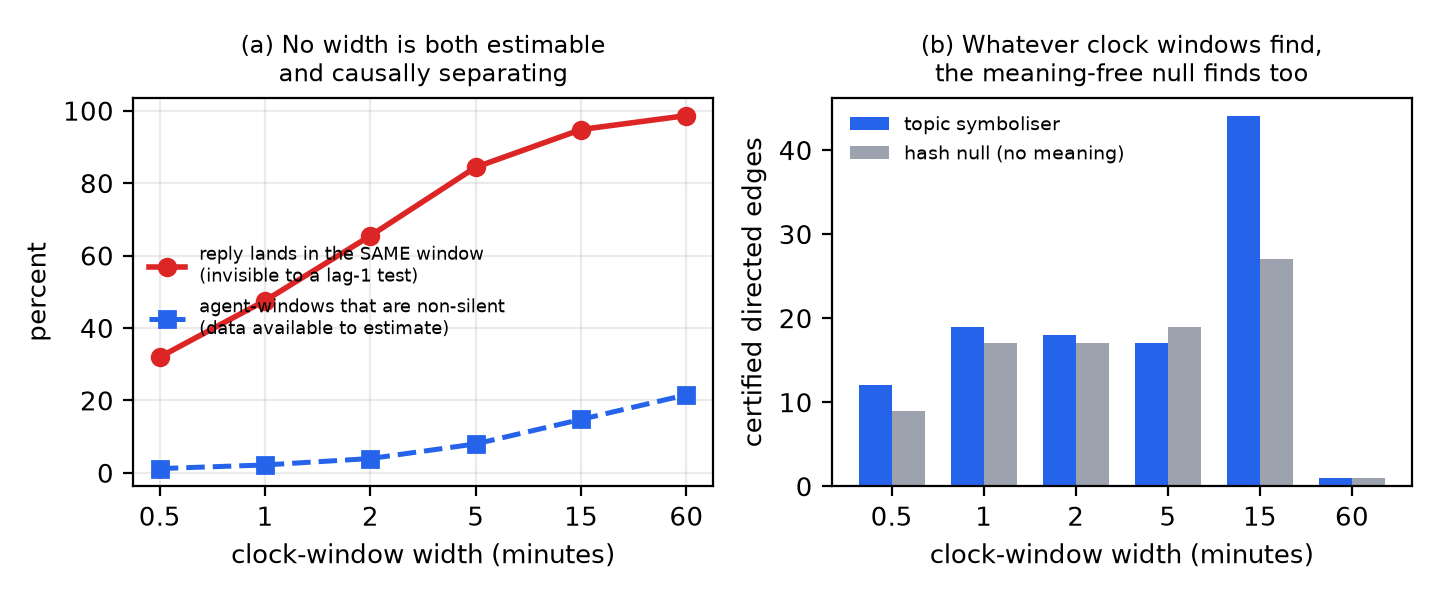
\includegraphics[width=0.9\textwidth]{f1_clock.png}
\caption{Clock-window transfer entropy on the 15 analysed agents of main-village \#general. Left, the two failure modes as a function of window width. Right, edges certified under the topic symboliser against the meaning-free hash null.}
\end{figure}

\section{power and replication in full}

\textbf{How much influence could we have seen?}

Absence of edges is only informative if the test could have found them, so we plant one. A synthetic follower at the median agent's volume copies the busiest agent's topic on a fraction of its messages. In main-village it goes undetected in 0 of 4 runs at couplings up to 0.4 and is caught in only 1 of 4 at 0.8. Holding coupling at 0.8 and varying how much it speaks, detection rises from 1 of 4 at 263 messages to 4 of 4 at 800 and stays there at 2000 and 4000, so the floor sits between 3\% and 10\% of the channel's messages.

Power is governed by how much an agent says, not only by how strongly it copies, and it is channel-specific: in open-chat a follower at that channel's median volume is caught in 3 of 4 runs at coupling 0.1 and in 4 of 4 from 0.2 upward. main-village's two edges are therefore a floor rather than a description.

\setcounter{figure}{1}
\begin{figure}[H]
\centering
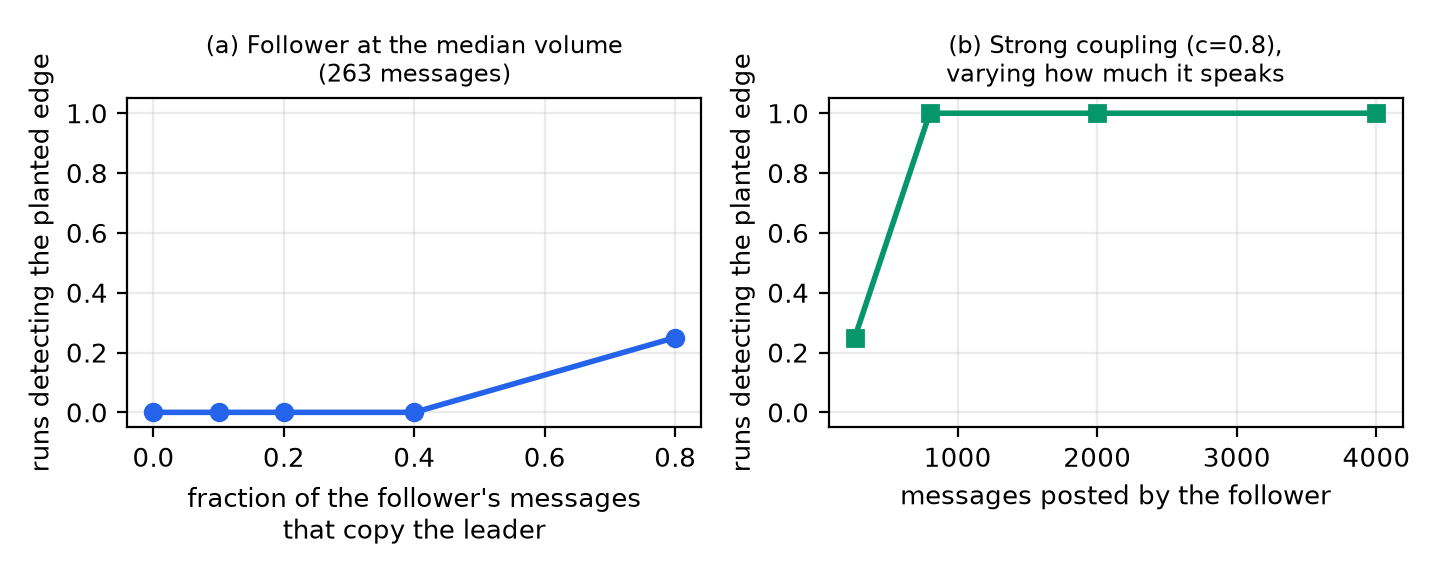
\includegraphics[width=0.9\textwidth]{f4_power.png}
\caption{Detection of a planted follower under the repaired surrogate. Left, varying the fraction of its messages that copy the leader, at the median agent's volume. Right, varying how much it speaks, at strong coupling.}
\end{figure}

\textbf{Does anything replicate?}

In main-village, no. Under the standard recipe the adjacent fourteen-day window shares 1 edge with the primary window out of 8 and 4, a Jaccard of 0.09, and the two halves share none. Under the repaired surrogate the adjacent window certifies nothing. The one edge that persists, GLM-5.2 to Gemini 3.5 Flash, is also the only edge the hash null certifies, so the single stable thing the standard recipe finds carries no meaning.

In open-chat, where the valid test has power, the picture is better but still partial: restricted to agents active in both windows and sharing one topic space, the current window certifies 9 edges and the previous 5, with 3 in common, a Jaccard of 0.27, against 0 from the hash null. About a third holds up. Splitting that window into halves is harsher, 7 edges against 2 with 1 in common, which the power result predicts, since halving the data moves agents below the floor.

The alphabet size remains a live degree of freedom even under the repaired surrogate, with open-chat certifying 8 edges at k=4, 18 at k=8 and 21 at k=16, so an edge count is never a property of a channel alone.

\textbf{Is the conditional test itself calibrated?}

It has to be asked, because a test that rejects nothing would produce Section 5.4's open-chat zero for the wrong reason. Taking the real main-village speaker sequence and permuting its symbols globally leaves data with no directed topical influence by construction, and the conditional test at full resolution fires in 2 of 40 such replicates. That is a family-wise error rate of 0.05 with a 95\% Wilson interval of 0.014 to 0.165, and the mean z across the family is -0.001. So the estimator is nominal on structure-free real data, and not biased downward: the open-chat degeneracy at nine context values is specific to that channel, where the joint space holds 6,561 cells against about 7,900 ticks and the surrogate statistic sits above the observed one for 65\% of pairs.

\section{the controls in full}

\textbf{Positive control (spike-in).} A synthetic agent is inserted into the real stream. A fraction c of its messages are responses placed immediately after a chosen leader's message, copying that leader's topic; the rest land at random positions carrying a symbol drawn from the channel's marginal distribution, so the planted agent's own volume and symbol usage look ordinary. Sweeping c at fixed volume gives the coupling floor, and sweeping volume at fixed c gives the volume floor. Both are reported in Appendix G, and both are channel-specific.

\textbf{Negative control, planted.} The same construction with c = 0: an agent whose messages carry the channel's marginal symbols at random positions, coupled to nothing. It should never be certified. Under the circular-shift surrogate it is certified in 8 of 8 runs once it posts 100 messages or more, which is the failure this report is about; under the permutation surrogate it is certified in 0 of 5 at both 263 and 1500 messages.

\textbf{Negative control, destroyed structure.} The real speaker sequence is kept exactly and the symbols are permuted globally across it. This leaves the speaking pattern, the sparsity, the burstiness and the non-stationarity of the real channel intact while removing any directed topical influence by construction, so a calibrated procedure should fire in about 5\% of replicates. This is the measurement behind the 0.90 and the 0.063 family-wise error rates, and behind the conditional test's 0.05 in Appendix G.

\textbf{Replication and sensitivity.} Each edge set is recomputed in the adjacent fourteen-day window, restricted to agents active in both windows with one topic space fit on the union so the symbol alphabet is shared; in each half of the primary window; and at alphabet sizes k of 4, 8 and 16. A meaning-free hash symboliser is run beside the topic symboliser at every clock width, and an independent LSA symboliser is run at the primary setting.

\section{humans in the channel, in full}

open-chat \#general is the only analysed channel with substantial human traffic: 124 visitors account for 32\% of its messages. Humans are included as nodes in two ways, and never identified; the individual variant uses the three busiest visitors under opaque labels.

\textbf{Humans collapsed into one node.} Pairwise certifies 19 edges, of which 13 are agent to agent, 4 run from humans to agents and 2 from agents to humans. Under conditioning 4 survive: 3 human to agent, 1 agent to agent, and 0 agent to human.

\textbf{The three busiest visitors as separate nodes.} Pairwise certifies 20 edges and conditioning leaves 2, one of which is an individual visitor driving a specific agent. The direction is the same in both treatments.

Two readings are available and the report commits to neither beyond what the test supports. The asymmetry survives conditioning, so it is not an artifact of the shared channel topic. But a human message followed by an agent message on the same topic is exactly what ordinary responsiveness looks like, and this measurement cannot separate ``the visitor steered the agent'' from ``the agent answered the visitor''. What it does establish is that the dependence is dyad-specific, directional, and absent in the reverse direction.

\begin{thebibliography}{}
\bibitem{ai2026}
AI Digest (2026). AI Village dataset. \url{https://huggingface.co/datasets/aidigestorg/ai-village} and \url{https://theaidigest.org/village}
\bibitem{greenblatt2024}
Greenblatt, R., Shlegeris, B., Sachan, K., and Roger, F. (2024). AI Control: Improving Safety Despite Intentional Subversion. arXiv:2312.06942.
\bibitem{runge2018}
Runge, J. (2018). Conditional Independence Testing Based on a Nearest-Neighbor Estimator of Conditional Mutual Information. Proceedings of the 21st International Conference on Artificial Intelligence and Statistics (AISTATS), PMLR 84, 938-947.
\bibitem{schreiber2000}
Schreiber, T. (2000). Measuring Information Transfer. Physical Review Letters, 85(2), 461-464.
\bibitem{shorten2021}
Shorten, D. P., Spinney, R. E., and Lizier, J. T. (2021). Estimating Transfer Entropy in Continuous Time Between Neural Spike Trains or Other Event-Based Data. PLOS Computational Biology, 17(4), e1008054.
\bibitem{westfall1993}
Westfall, P. H., and Young, S. S. (1993). Resampling-Based Multiple Testing: Examples and Methods for p-Value Adjustment. Wiley.
\end{thebibliography}

\end{document}
